\documentclass[12pt,a4paper]{article}
\usepackage{cite}
\usepackage{fullpage}
\usepackage{indentfirst}
\usepackage{parskip}
\usepackage{amsmath}
\usepackage{hyperref}
\usepackage{bm}
\usepackage{enumerate}
\usepackage{enumitem}
\usepackage{graphicx}
\usepackage{booktabs}
\usepackage{url}
\usepackage{textcomp}
\usepackage{iitem}
\usepackage{ragged2e}
\usepackage[UTF8]{ctex}

\begin{document}
\justifying
\setlength{\parindent}{2em}

\pdfbookmark[0]{Front page}{label:frontpage}%
\begin{titlepage}
  \noindent%
  \begin{tabular}{@{}p{\textwidth}@{}}
    \toprule[2pt]
    \midrule
    \vspace{0.2cm}\\
    \begin{center}
    \Huge{\textbf{
      分布式存储与计算项目报告 \\[8pt]
    }}
    \end{center}
    \begin{center}
      \Large{
        分布式计算课程期末项目
      }
    \end{center}
    \vspace{0.2cm}\\
    \midrule
    \toprule[2pt]
  \end{tabular}
  \vspace{5 cm}
  \begin{center}
    {\Large
      第15组
    }\\
    \vspace{0.2cm}
    {\Large
      1831605 \quad 刘诗洋 \\[5pt]
      1831606 \quad 陆思远 \\[5pt]
      1831607 \quad 余\quad豪 \\[5pt]
    }
  \end{center}
  \vfill
  \begin{center}
    {\Large
      同济大学\\[5pt]
      软件学院\\[5pt]
    }
  \end{center}
\end{titlepage}
\clearpage

\tableofcontents
\clearpage

\section{项目需求}
本项目需要设计和实现一个由多个节点组成的分布式系统,完成分布式存储和分布式计算的功能。节点数目不能低于4个,可以是虚拟机或实体机。
\subsection{分布式存储}
分布式存储模块要求实现基本的存储功能,包括:
\begin{enumerate}
	\item 文件的分块与备份。系统对大容量文件以分块的形式存储,并且系统中
	存储的每个文件都有多个副本,当系统中不超过 20\%的节点失效时,也
	不影响系统中所有文件的访问。 
	\item 文件的一致性。从任意一个节点访问并更新某个文件后,其在系统中的
	副本也相应进行更新。 
\end{enumerate}
\subsection{分布式计算}
分布式计算模块需要使用分布式系统的计算资源来处理以下事物:
\begin{enumerate}
	\item 计算出用户的每日平均通话次数,并将结果以$<$主叫号码, 每日平均通话次数$>$的格式保存成txt或excel文件。
	\item 计算出不同通话类型(市话、长途、国际)下各个运营商(移动,联通,电信)的占比,并画出饼状图。 
	\item 计算出用户在各个时间段(时间段的划分如表1所示)通话时长所占比例,并将结果以$<$主叫号码, 时间段1占比, \ldots, 时间段8占比$>$的格式保存成txt或excel文件。
\end{enumerate}

\begin{table}[htb]
\caption{时间段划分表}
\centering
\begin{tabular}{c c}
\label{time period}
\\
\hline
\hline
\textbf{时间段名称} ~ & ~ \textbf{时间段的起止时间} \\[6pt]
\hline
时间段1 ~ & ~ 0:00-3:00 \\[6pt]
\hline
时间段2 ~ & ~ 3:00-6:00 \\[6pt]
\hline
时间段3 ~ & ~ 6:00-9:00 \\[6pt]
\hline
时间段4 ~ & ~ 9:00-12:00 \\[6pt]
\hline
时间段5 ~ & ~ 12:00-15:00 \\[6pt]
\hline
时间段6 ~ & ~ 15:00-18:00 \\[6pt]
\hline
时间段7 ~ & ~ 18:00-21:00 \\[6pt]
\hline
时间段8 ~ & ~ 21:00-24:00 \\[6pt]
\hline
\hline
\end{tabular}
\end{table}

\clearpage

\section{项目分析与设计}
项目需要建立分布式的节点,并可以从任一节点获取文件。我们的设计思路为将存储/计算任务节点与事务处理节点分离,这两部分都可形成分布式。最后,再使用接口的形式,向客户端(web页面)暴露功能。这样即可达到可扩展性、容错性等分布式需求。具体到功能,有如下设计方案。
\subsection{文件分块与备份}
根据每个存储节点的容量,我们可以自定义分块大小,如$128$Mb,$64$Mb,并使用多线程的方式对待上传文件进行切分。另外,备份数目也可做调整,按照项目要求的容错性,当不超过$20\%$节点宕机时,系统依然可以正常运行。那么,假设每个节点均独立分布且宕机概率一致,则对于$N$个节点的系统来说,每个文件块至少需要
\begin{equation}
\lfloor 0.2N \rfloor+1
\end{equation}
个备份。例如我们在测试过程中使用了4个存储节点,则需要$2$个备份。 当然,在实际的分布式存储项目中,不同节点间的宕机概率不是独立的,很难会出现同时存储同一数据块的节点全部失效的情况。

在存储过程中,我们会考虑存储节点的存储空间,优先将文件块存储在可用空间更多的节点上。这样做的优点是使得不同的存储节点存储压力会较为均衡,而不至于出现有些节点存储内容过多而另一些空闲的不平衡情况。
\subsection{文件一致性保证}
首先,我们会检测上传文件的文件名是否已经存在于文件系统中,若以存在,则以更新的方式进行上传。对于存在修改的内容,系统会先将存储节点的相应备份删除,再重新写入新内容。这一操作对所有文件块都会执行,所以保证了文件的一致性。

另外,在系统运行时,用户能实时获取到所有存储节点和文件系统中所有文件的状态,包括节点是否在线、文件是否完整、文件所处的节点位置等。当然,在实际的云存储系统中,不同用户的权限是不同的,对同一份文件,有的用户是可写,而有的用户仅为可读。在我们的测试系统中,暂不考虑用户权限,仅展示可操作功能。

\section{系统实现}
\subsection{分布式存储}
\subsubsection{整体框架}
整个分布式存储系统有三层结构,分别为:用户访问层,事务处理层以及文件存储层。每层间仅能与相邻层通信,也即用户无法直接对文件存储节点进行操作,这样保证了文件的安全性。每层均为分布式的结构,也即用户可通过web接口访问系统,无论他位于何处;事务处理层有若干独立分布的服务器,用于处理用户的请求。一般来说,分布式的服务有两个目的:一是负载均衡,将服务分发至合适的节点上执行;二是将不同的服务部署在不同的节点上,但节点间的服务可相互调用。如在本项目中,我们可以将存储服务、下载服务与文件系统更新服务分离,但它们之间是可以相互访问的。现在有许多架构可实现这样的分布式服务,如Apache Dubbo等,限于时间,我们未将精力放在这一实现上。图\ref{storage_architecture}展示了分布式存储模块的系统架构。
\subsubsection{文件切片}
切片函数使用多线程,每$64$Mb切分为一块,并命名为filename.format.ID.part. 若文件小于$64$Mb,则不进行切分。
\subsubsection{文件上传}
我们通过SCP(Secure copy),跨机远程拷贝来进行请求服务节点和存储节点间的文件传输。在服务节点上,使用java的SCPClient来调用putFile()和getFile()。当然,在上传前,系统会检测该文件是新文件(即系统中不存在)或是更新的文件(即系统中有旧版本),若存在旧版本,则会先将旧版本文件块删除后,再上传新的文件块。
\subsubsection{文件备份}
为了增加存储系统的安全性,我们设置了冗余机制——对每份文件增加一份备份,并保存在不同的存储节点中。在下载文件时,我们按datanode的序号顺序对block进行搜索,直至找到该文件的完整的一份blocks。再在本地进行merge,更新等操作。
\subsubsection{文件下载}
当用户发出下载请求时,系统会将相应的文件块从存储节点中获取到并下载,拼接完成后返回给用户。
\subsubsection{存储系统状态查看}
为了监控存储系统的节点状态和文件状态,用户可以通过接口查看这些信息。系统会定时与存储节点进行通信,若连续未收到某存储节点的回复,则认为其处于宕机状态。另外,当用户查看文件时,根据当前的存储节点健康状况,系统会检测该文件各个区块是否还可获得以及整个文件是否还完整。
\subsubsection{存储系统文件管理}
使用Java序列化的机制,将系统中的文件信息保存于日志中,当需要对其更新时(如上传文件时),再对文件反序列化,将其更新后再序列化为文件。这样即可保存一个完整的系统信息。
\subsubsection{系统优化:存储负载均衡}
我们还考虑了这个系统的负载均衡——保证各个存储节点间存储负荷相对平衡。这就要求在将block存至DataNode中时,考虑存储节点的实际剩余空间。在每次提交一个block(及其备份时),我们选择当前剩余空间最大的两个DataNode,将其存储进去。


\begin{figure}[htb]
\centering
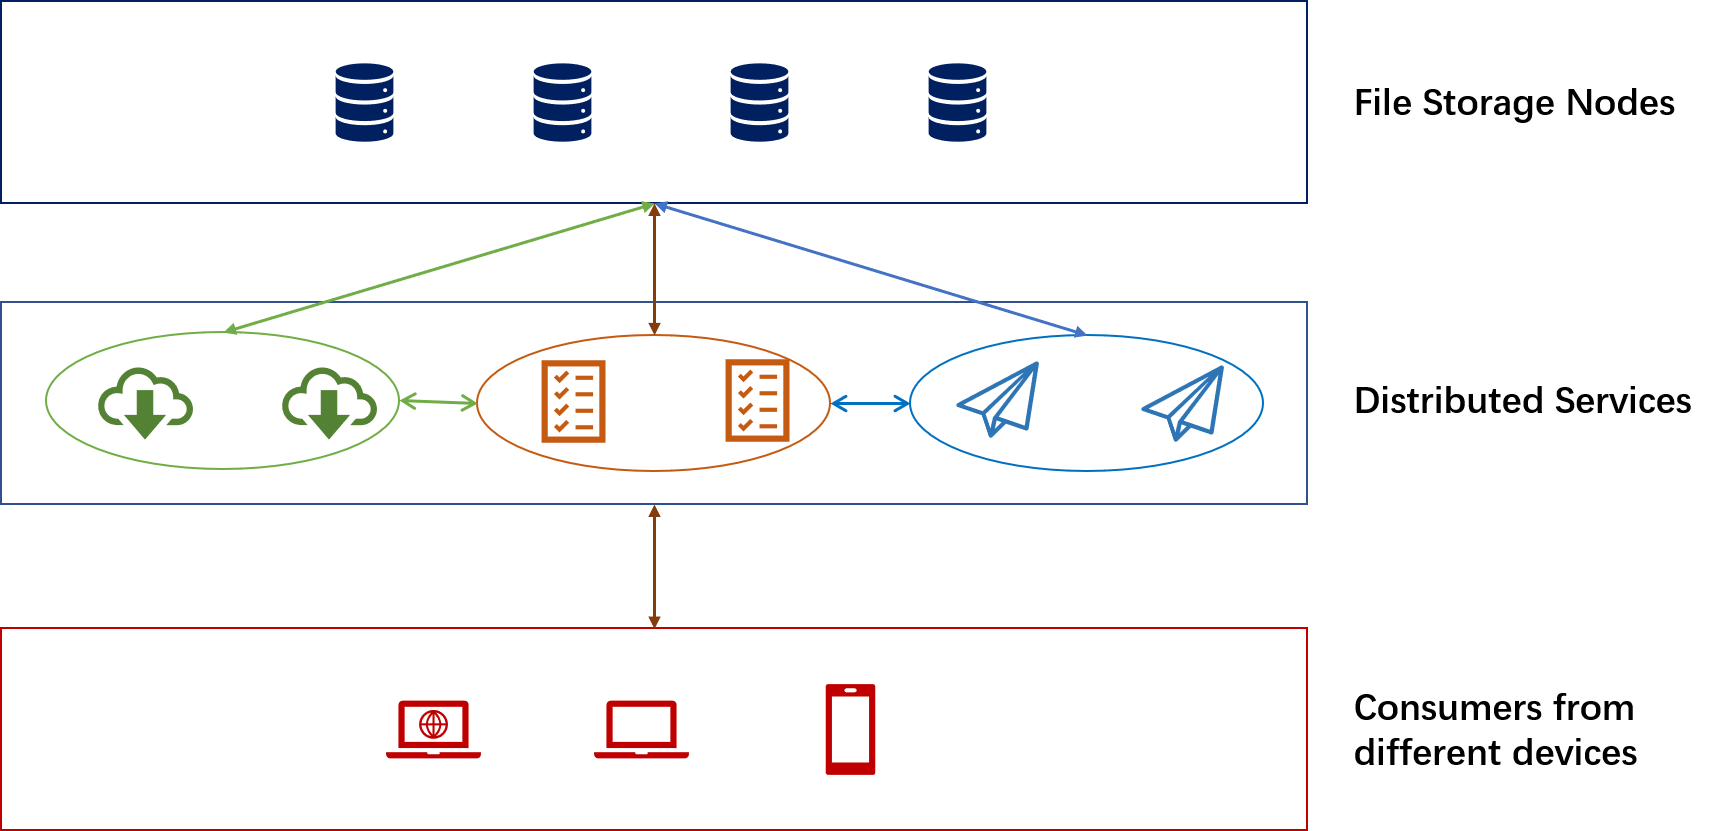
\includegraphics[width=14cm]{storage_architecture}
\caption{分布式存储系统架构 \label{storage_architecture}}
\end{figure}

\clearpage

\subsection{分布式计算}
\subsubsection{整体框架}
基于Hadoop HDFS搭建了Spark分布式的内存并行计算引擎框架,由于其是基于内存进行运算的,即每次shuffle操作后,无需写到磁盘,可以缓存在内存中,因而其处理速度更快,相比传统的MapReduce而言更加高效,弥补了MapReduce的不足。

为了完成数据分析和统计的工作,决定采用Spark SQL模块,主要用于进行结构化数据的处理。它提供的最核心的编程抽象就是DataFrame,DataFrame可以根据很多种源数据进行构建,包括:结构化的数据文件,Hive中的数据表,外部的关系型数据库,以及RDD(弹性分布式数据集)即Spark中的最基本的数据抽象。

在本项目中,利用Pyspark进行并行计算,基本工作流程和结构如图\ref{computing_architecture}所示:

\begin{figure}[htb]
\centering
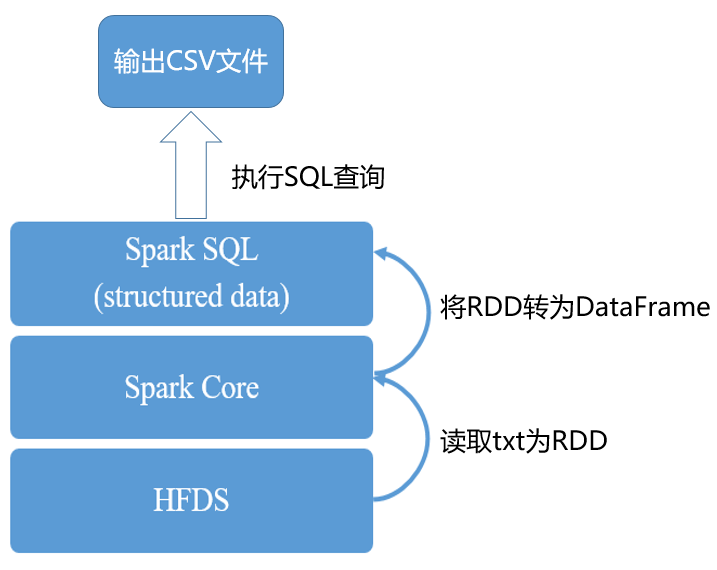
\includegraphics[width=10cm]{computing_architecture}
\caption{分布式计算系统架构 \label{computing_architecture}}
\end{figure}
\subsubsection{源数据解析}
待处理的源数据文件“tb\_call\_201202\_random.txt”分布式得存储在Hadoop HDFS中,Spark读取源数据文件为RDD,需要构造Map函数对源数据文件进行解析,该解析函数为自己定义的函数(对每一行数据进行$split()$操作)。
\subsubsection{时间段计算}
由于在Spark SQL中不支持进行原生SQL语句中的时间差计算的函数timediff,因而需要在执行SQL语句前对每一次的通话过程进行切分,将其划分到不同的时间段,此处需要对跨天的通话进行特别处理。这种情况下需要定义时间切分函数,并将其注册为udf,来对DataFrame进行解析。

例如对于如下的时间段,会有相应切分(图\ref{time_period}):
\begin{figure}[htb]
\centering
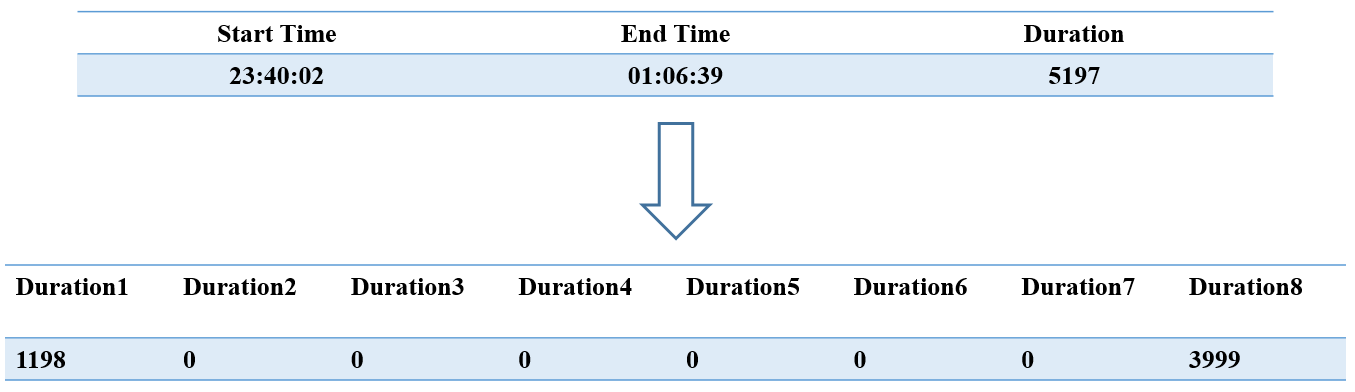
\includegraphics[width=14cm]{time_period}
\caption{时间段切分 \label{time_period}}
\end{figure}

为了能将RDD转化为DataFrame格式,需要自定义schema来指定StructField(包括字段名和字段类型),根据需求可以有schema,包含原本的14个字段以及附加的8个字段(用来表示该次通话在该时间段中的通话时长),StructField有如下的形式:

\begin{equation}
StructField(\mathrm{"day\_id",\ StringType(),True})
\end{equation}

构造完DataFrame后还需利用函数$createOrReplaceTempView()$将DataFrame注册为临时表(临时视图),这样就可以通过简单的$Spark.sql$语句利用$SUM$或者$COUNT$进行统计操作,最后将SQL查询结果的DataFrame以csv格式进行存储到本地。

\subsubsection{问题求解}
\begin{enumerate}
\item 用户的每日平均通话次数(图\ref{sql_1})
\begin{figure}[htb]
\centering
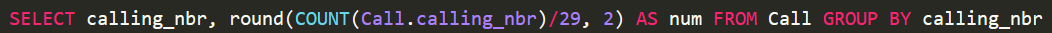
\includegraphics[width=14cm]{sql_1}
\caption{SQL: 用户的每日平均通话次数 \label{sql_1}}
\end{figure}

\item 同通话类型下各个运营商的占比(图\ref{sql_2})
\begin{figure}[htb]
\centering
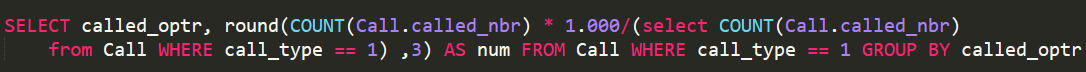
\includegraphics[width=14cm]{sql_2}
\caption{SQL: 同通话类型下各个运营商的占比 \label{sql_2}}
\end{figure}

\item 用户在各个时间段通话时长的占比(图\ref{sql_3})
\begin{figure}[htb]
\centering
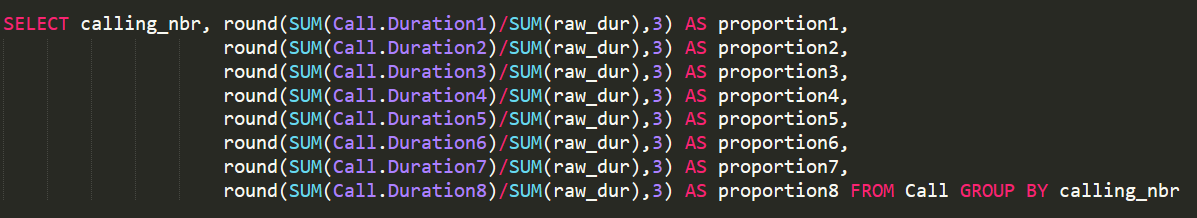
\includegraphics[width=14cm]{sql_3}
\caption{SQL: 用户在各个时间段通话时长的占比 \label{sql_3}}
\end{figure}

\end{enumerate}

\section{系统运行与结果}
\subsection{分布式存储}

\subsubsection{文件上传}
用户可通过浏览器,选择想要上传的文件,如图\ref{upload_1}所示。当文件上传完毕后,会有相应的提示(图\ref{upload_2})。
\begin{figure}[htb]
\centering
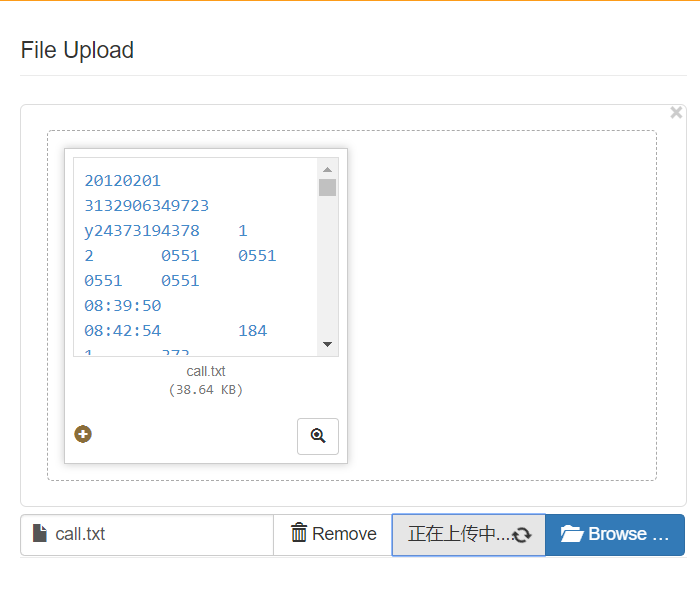
\includegraphics[width=14cm]{upload_1}
\caption{选择文件并上传 \label{upload_1}}
\end{figure}
\begin{figure}[htb]
\centering
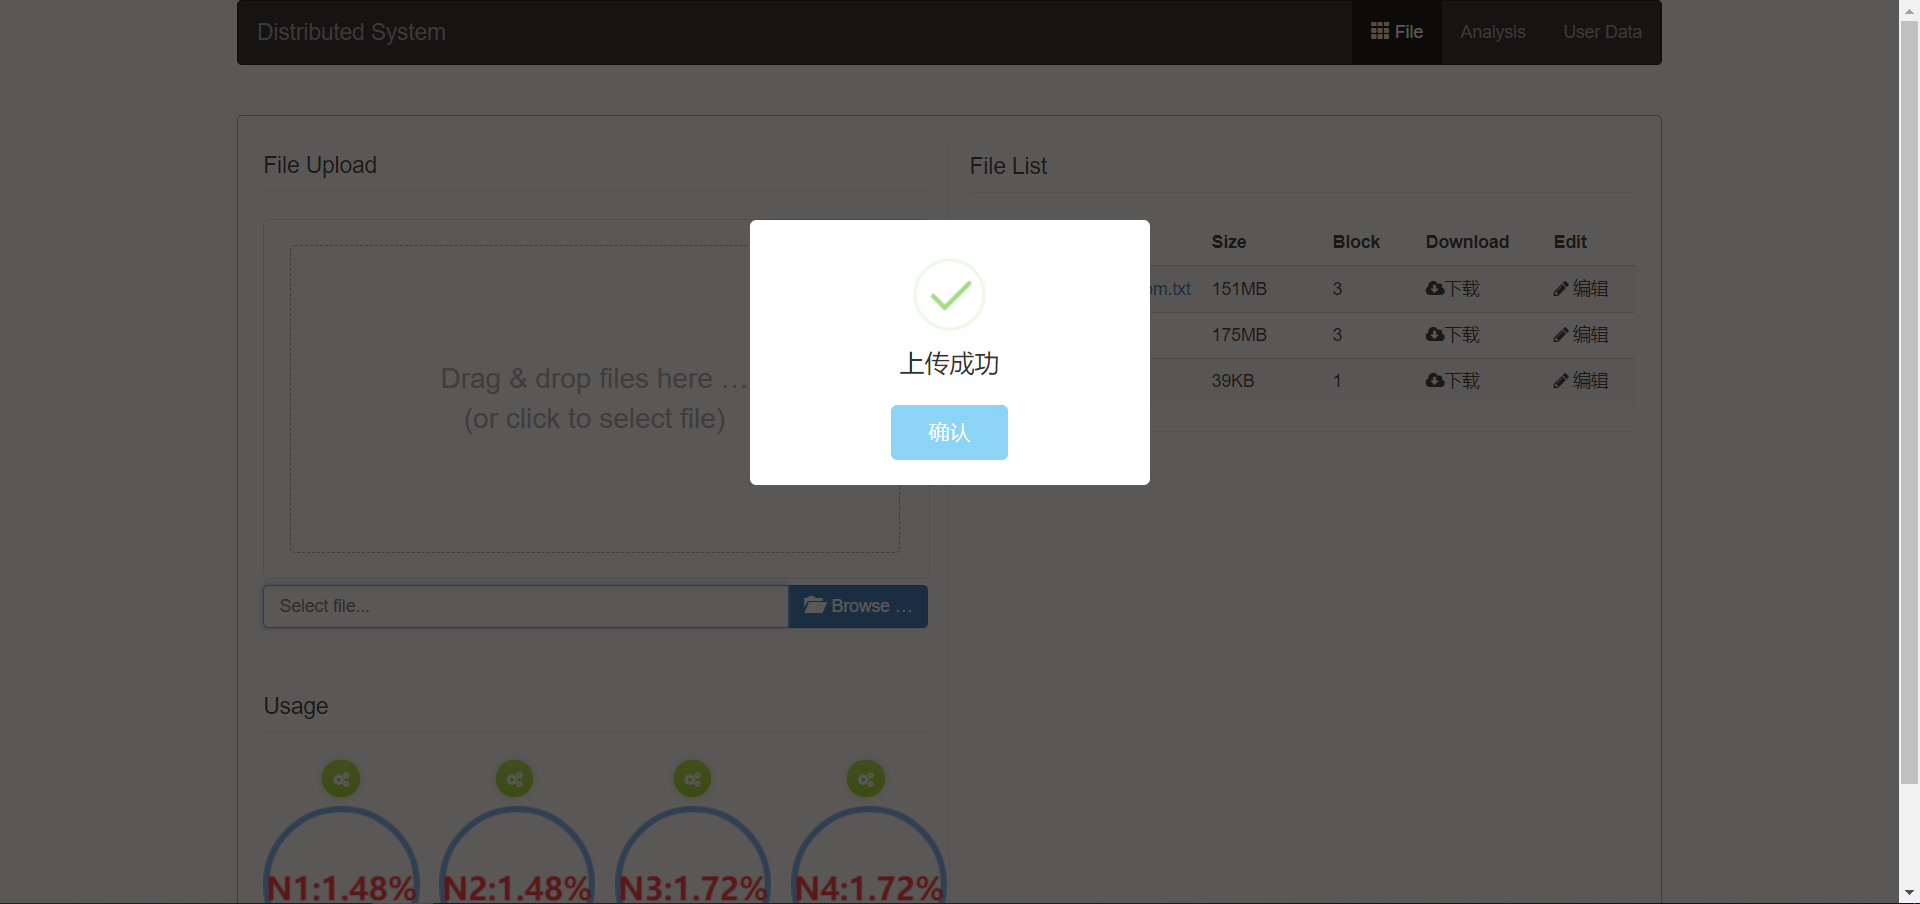
\includegraphics[width=14cm]{upload_2}
\caption{上传成功提示 \label{upload_2}}
\end{figure}

\subsubsection{查看文件列表}
每次上传文件、删除文件、编辑文件后文件列表会自动更新
文件列表中显示包括文件名、文件大小、文件的block数以及下载和编辑(文本更新和删除)的选项。(图\ref{list_1})
\begin{figure}[htb]
\centering
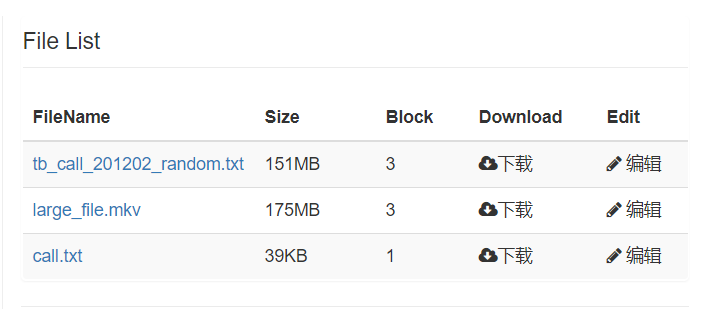
\includegraphics[width=14cm]{list_1}
\caption{查看文件列表 \label{list_1}}
\end{figure}

\subsubsection{查看文件详情}
文件详情包括文件当前状态(即文件是否完好)以及文件block及其副本在各个结点上存储的大小。(图\ref{detail_1})
\begin{figure}[htb]
\centering
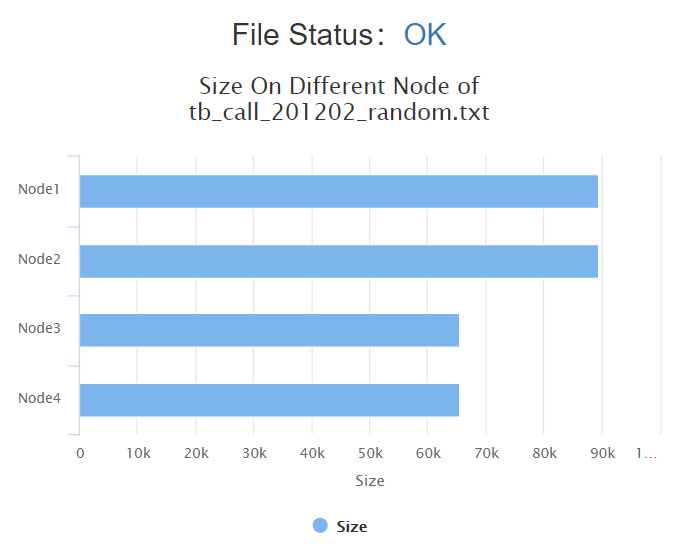
\includegraphics[width=14cm]{detail_1}
\caption{查看文件详情 \label{detail_1}}
\end{figure}

\subsubsection{文件下载}
在文件列表中,用户可选择相应的文件并点击右侧的下载按钮进行下载,下载完毕后,文件经有浏览器的下载控件保存至本地。(图\ref{download_1})
\begin{figure}[htb]
\centering
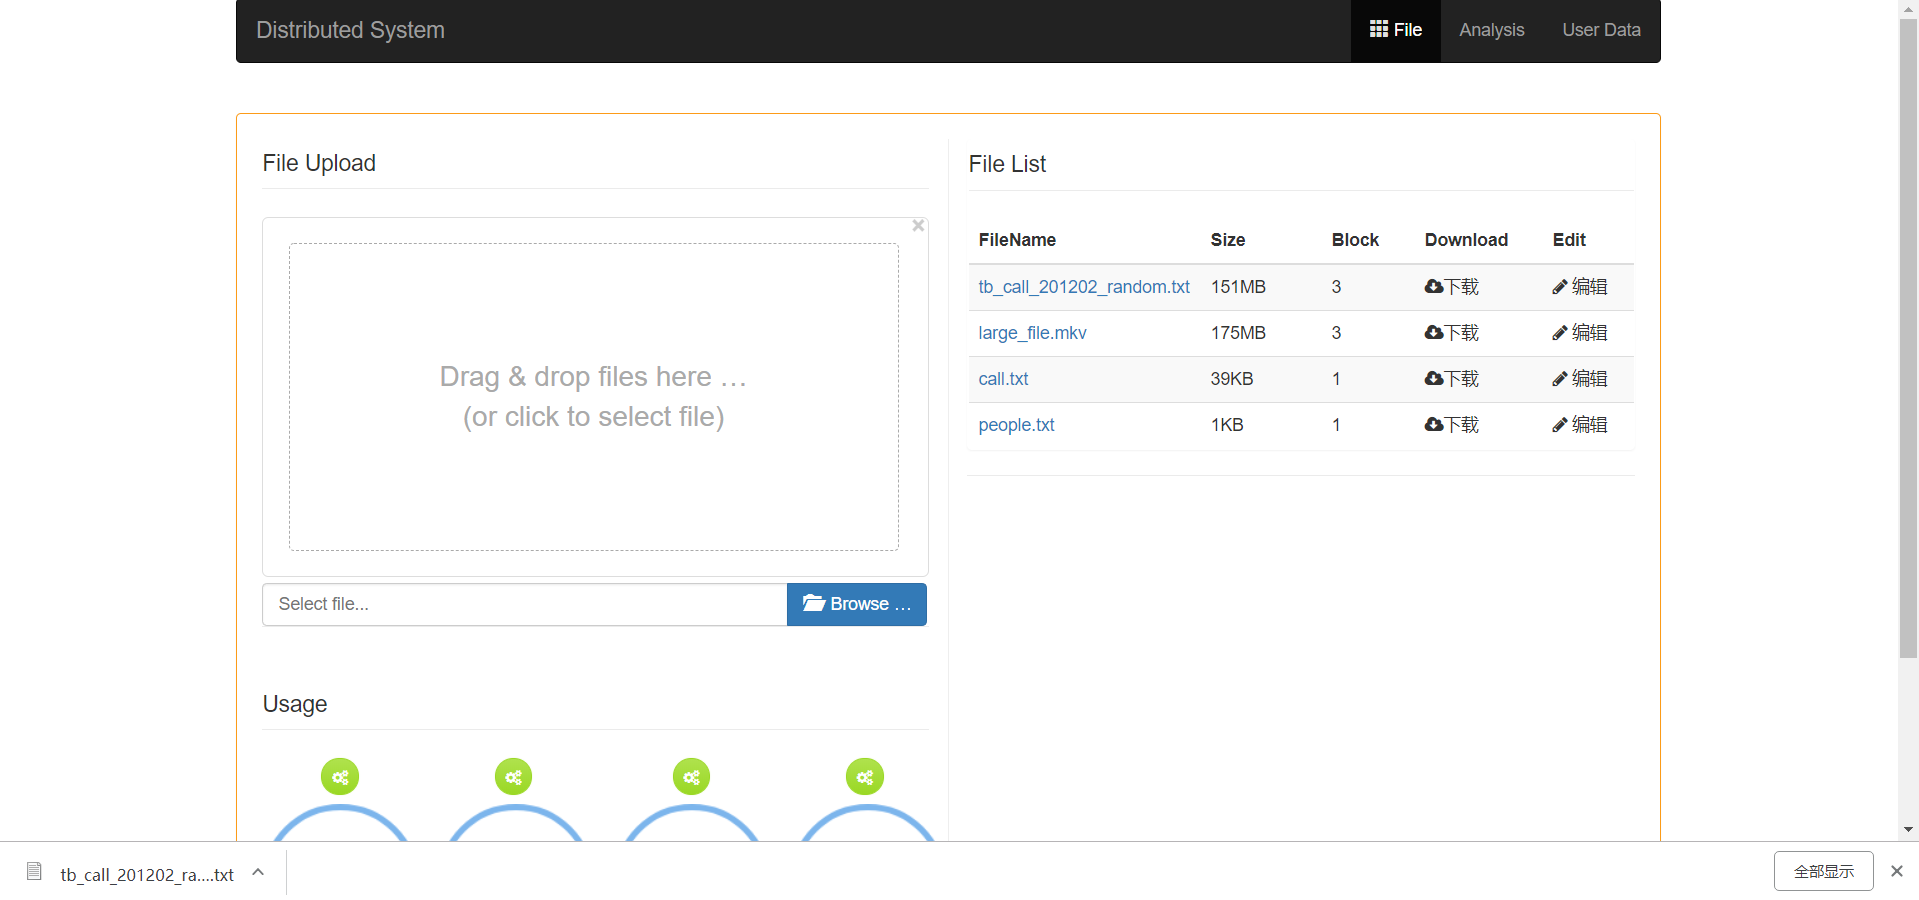
\includegraphics[width=14cm]{download_1}
\caption{文件下载 \label{download_1}}
\end{figure}

\subsubsection{文件编辑与更新}
对于文本类文件,系统还可支持在线编辑并更新。(图\ref{update_1})
\begin{figure}[htb]
\centering
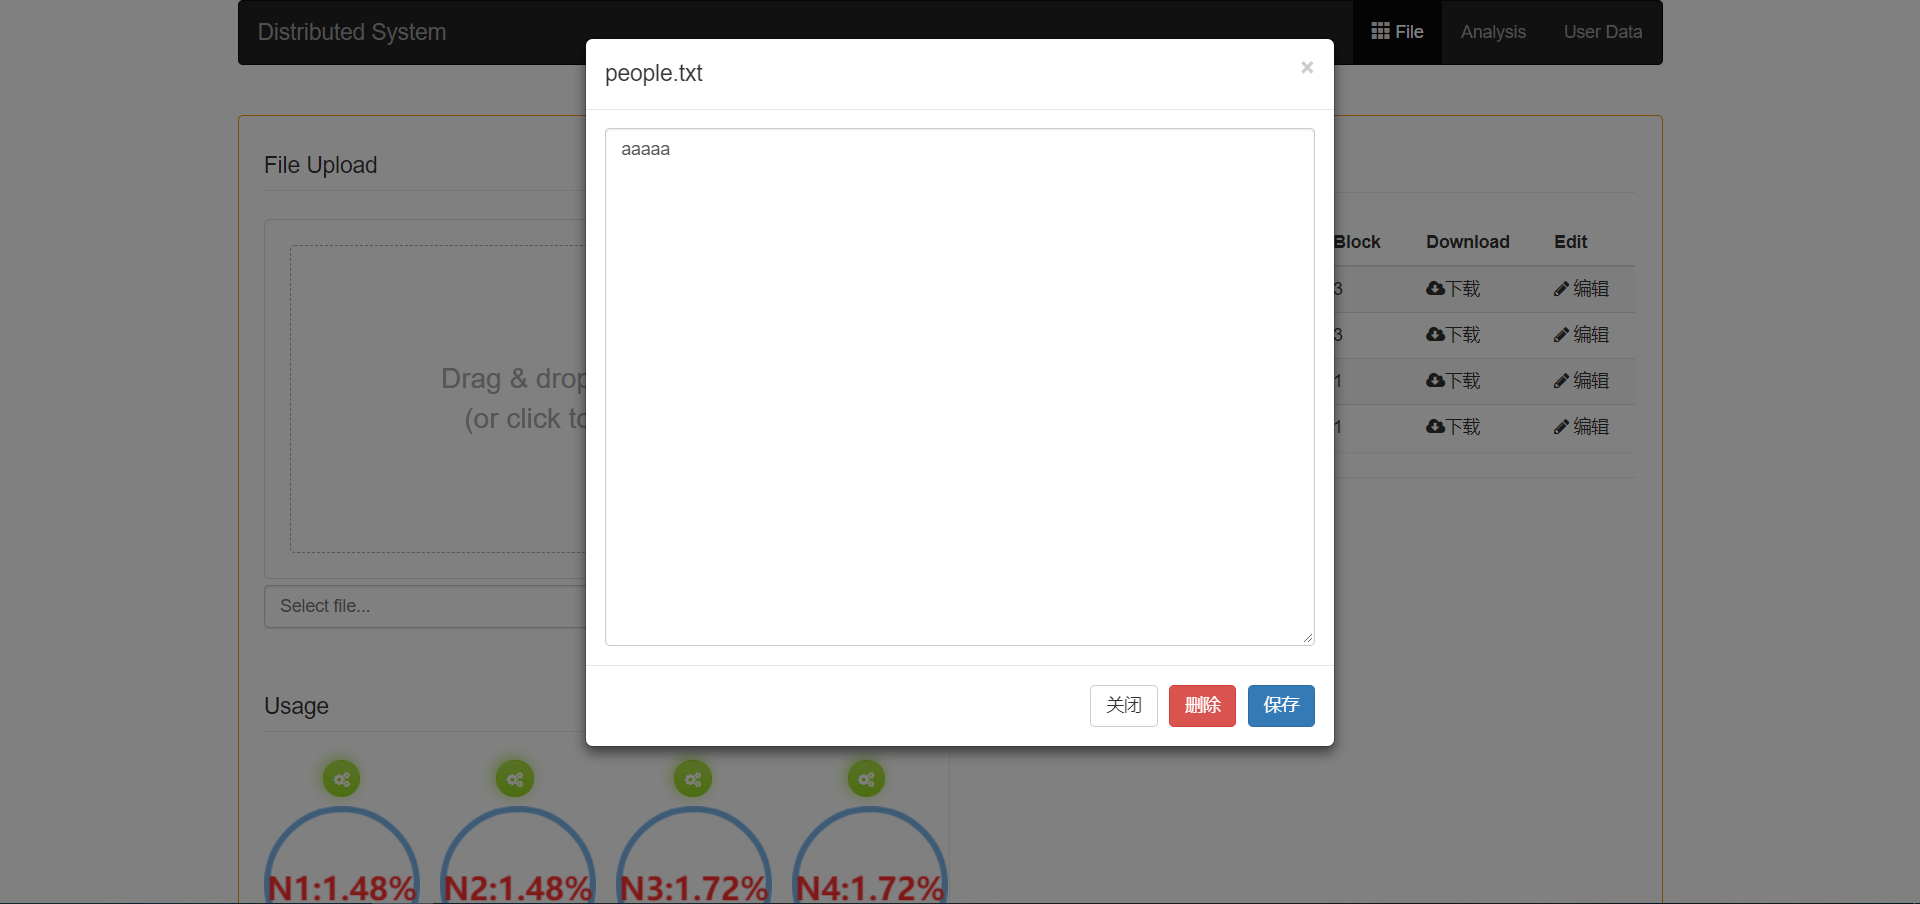
\includegraphics[width=14cm]{update_1}
\caption{文件编辑并更新 \label{update_1}}
\end{figure}

\subsubsection{文件删除}
删除文件后,系统将更新文件列表即节点存储空间。(图\ref{delete_1})
\begin{figure}[htb]
\centering
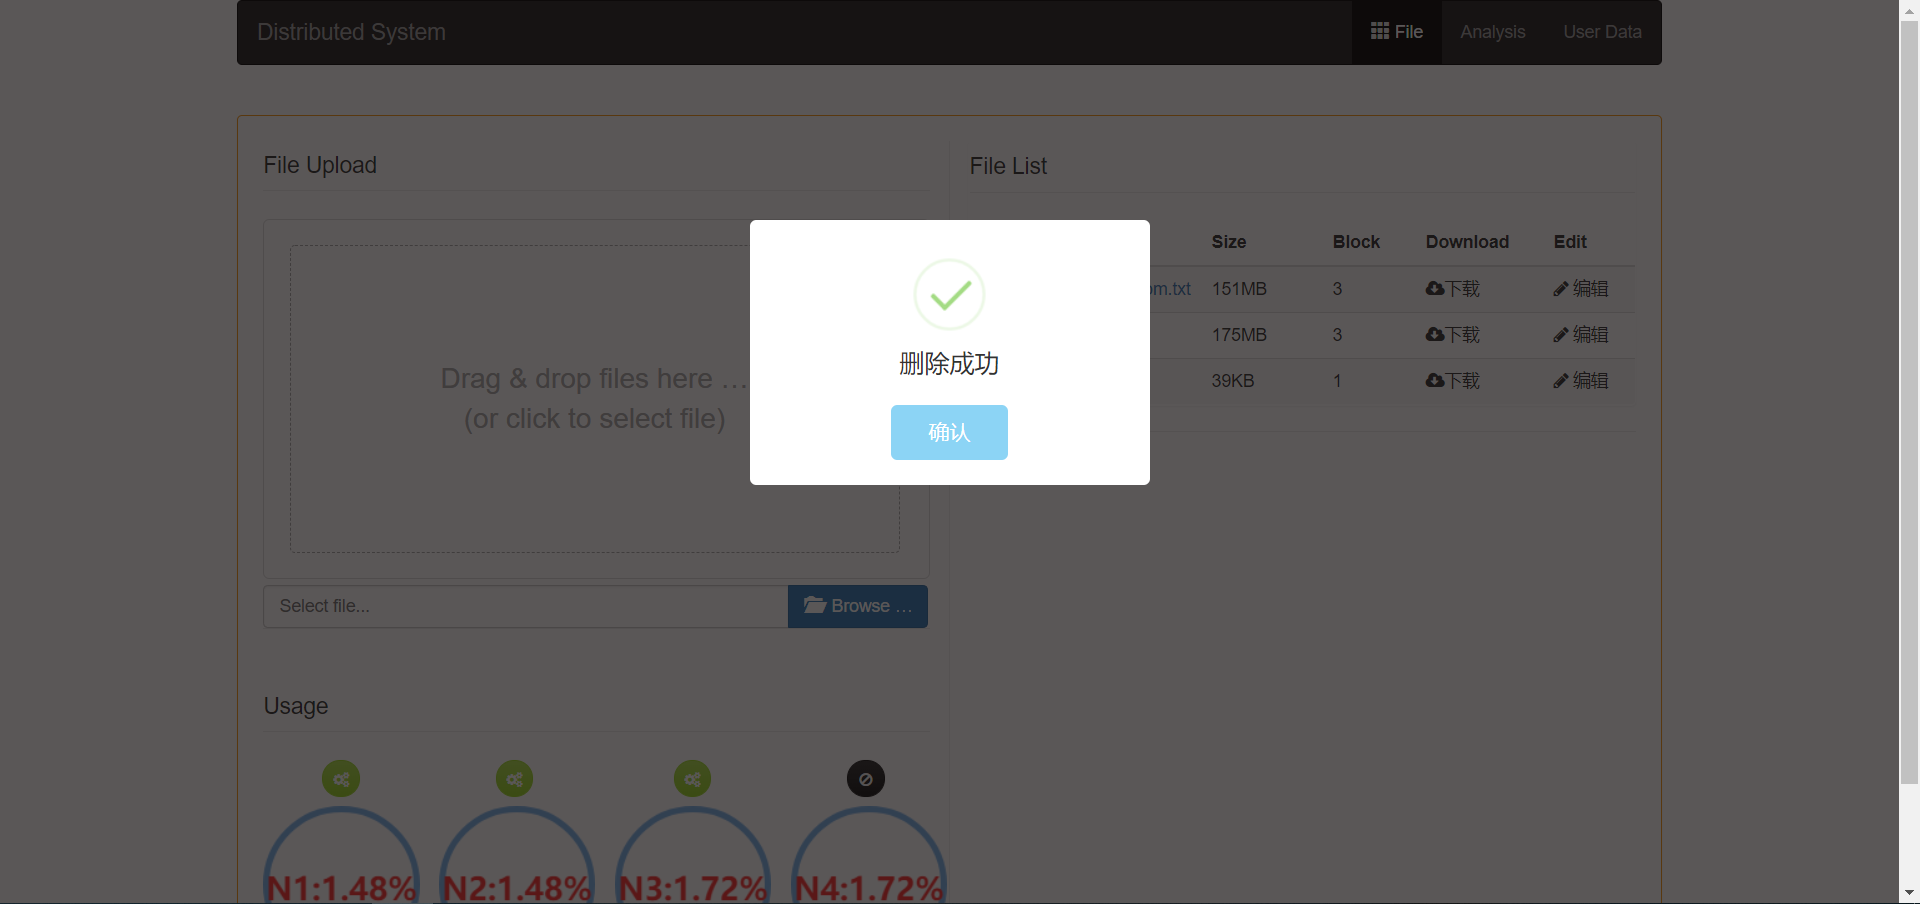
\includegraphics[width=14cm]{delete_1}
\caption{文件删除 \label{delete_1}}
\end{figure}

\subsubsection{节点状态与文件完整性监控}
节点状态:绿色表示节点启动完好,黑色表示节点挂起或失效。Bubble中的百分比表示节点的存储的使用量。(图\ref{node_1})
\begin{figure}[htb]
\centering
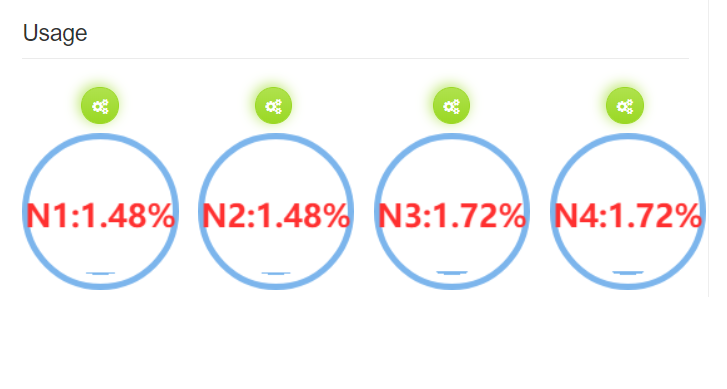
\includegraphics[width=14cm]{node_1}
\caption{节点状态 \label{node_1}}
\end{figure}

此时有25\%的节点宕机或者挂起,那么文件依然能够读取,状态为有效。(图\ref{node_2},\ref{node_3})
\begin{figure}[htb]
\centering
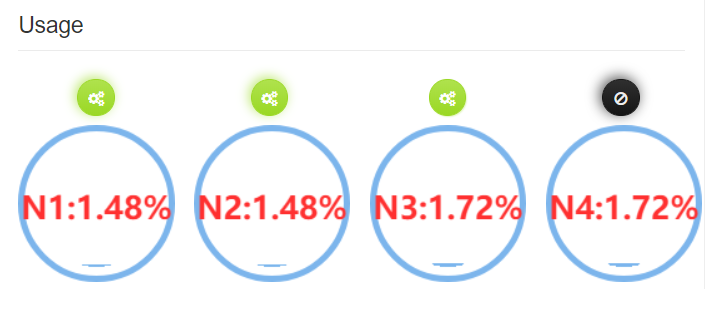
\includegraphics[width=14cm]{node_2}
\caption{节点状态(有一个节点宕机) \label{node_2}}
\end{figure}

\begin{figure}[htb]
\centering
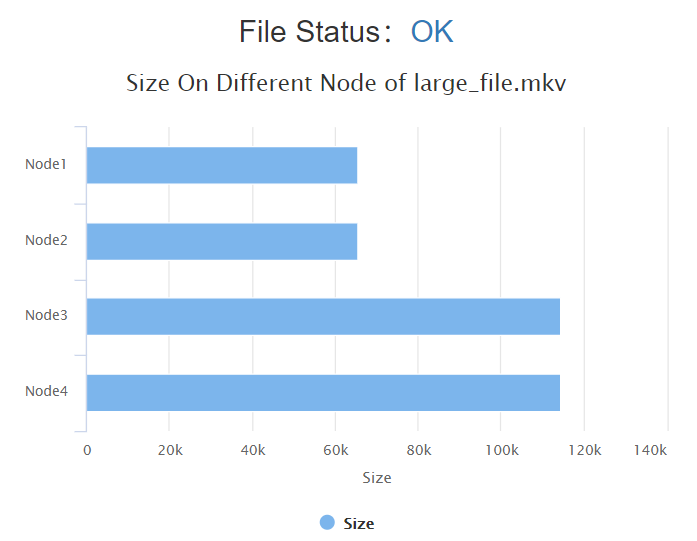
\includegraphics[width=14cm]{node_3}
\caption{节点状态(有一个节点宕机),文件依然完整 \label{node_3}}
\end{figure}

此时有一半的节点宕机或者挂起(超过25\%),那么则会有文件无法读取,状态为失效。(图\ref{node_4},\ref{node_5})

\begin{figure}[htb]
\centering
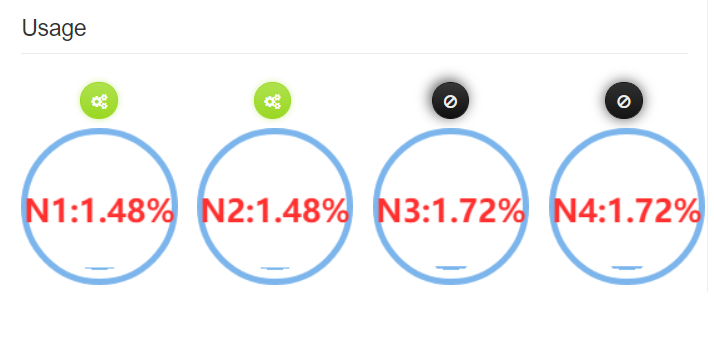
\includegraphics[width=14cm]{node_4}
\caption{节点状态(有两个节点宕机) \label{node_4}}
\end{figure}

\begin{figure}[htb]
\centering
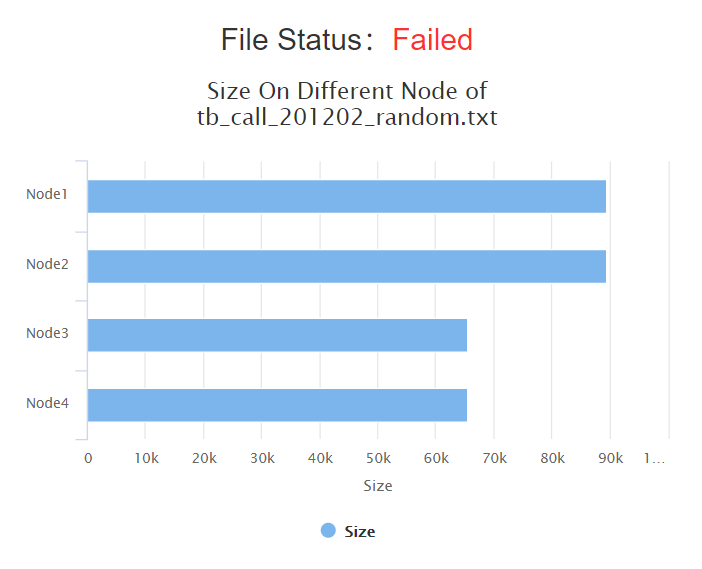
\includegraphics[width=14cm]{node_5}
\caption{节点状态(有两个节点宕机),文件不完整 \label{node_5}}
\end{figure}

\clearpage

\subsection{分布式计算}
分布式计算的结果,我们以饼图(图\ref{computing_result_1},\ref{computing_result_2},\ref{computing_result_3},\ref{duration_distribution})和折线图(\ref{month_num})表示。另外,详细结果也将提交在csv文件中。
\begin{figure}[htb]
\centering
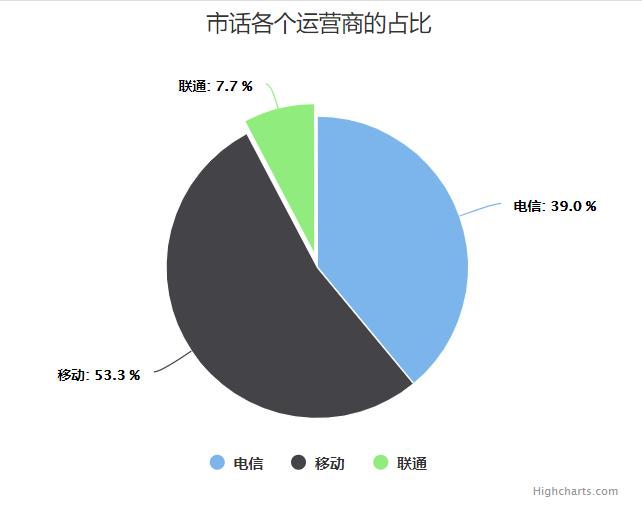
\includegraphics[width=10cm]{computing_result_1}
\caption{市话各运营商占比 \label{computing_result_1}}
\end{figure}
\begin{figure}[htb]
\centering
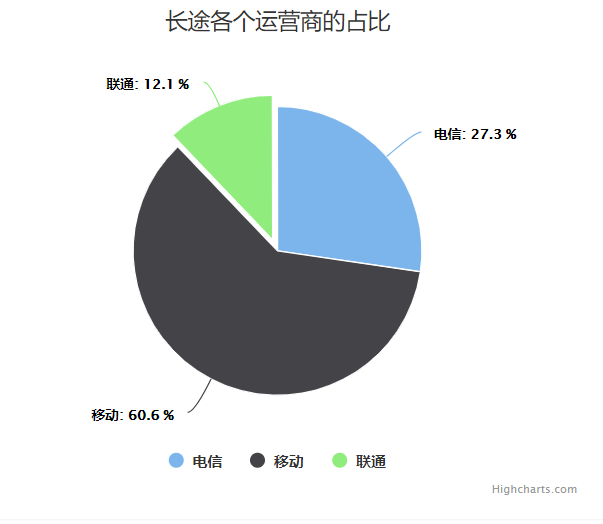
\includegraphics[width=10cm]{computing_result_2}
\caption{长途各运营商占比 \label{computing_result_2}}
\end{figure}
\begin{figure}[htb]
\centering
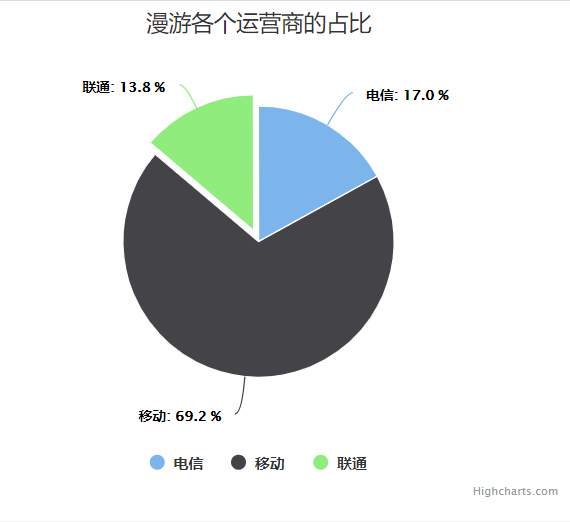
\includegraphics[width=10cm]{computing_result_3}
\caption{漫游各运营商占比 \label{computing_result_3}}
\end{figure}
\begin{figure}[htb]
\centering
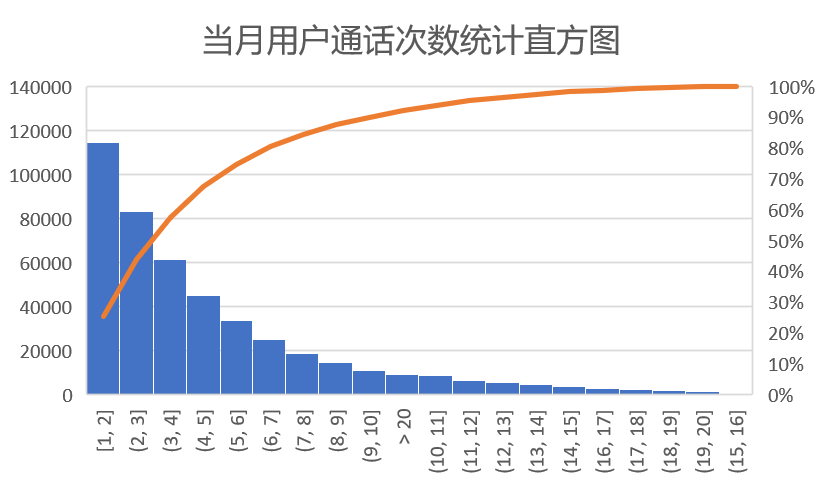
\includegraphics[width=10cm]{month_num}
\caption{当月用户通话次数统计 \label{month_num}}
\end{figure}
\begin{figure}[htb]
\centering
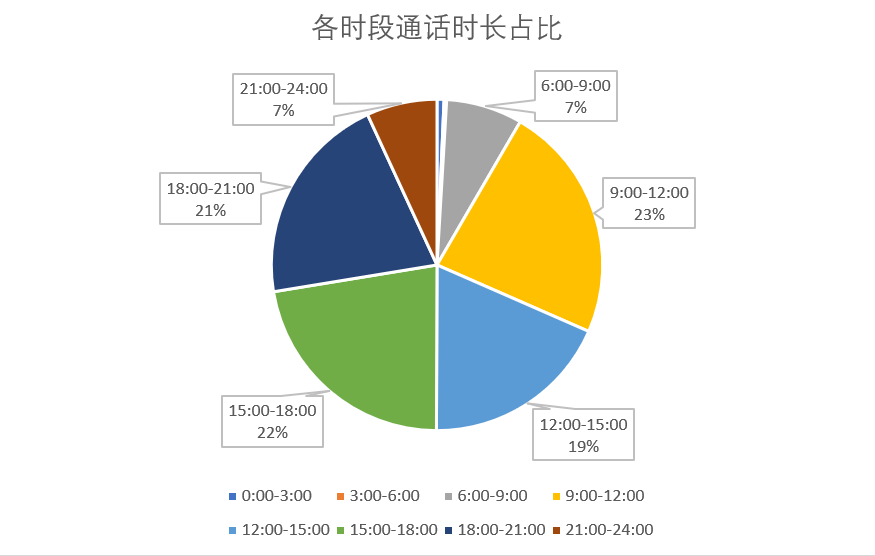
\includegraphics[width=10cm]{duration_distribution}
\caption{各时段通话时长占比 \label{duration_distribution}}
\end{figure}

\section{总结}
该项目中,我们设计并实现了分布式文件存储系统,以及利用Hadoop和Spark计算框架实现了分布式计算。尽管整个项目还很粗糙,有许多功能还未完善,但重在思考在分布式存储和计算中的框架设计。通过这次项目,我们对分布式存储和计算过程中的任务分配、状态管理、一致性管理等方面都有了更多的思考。

\section{提交内容}
\begin{itemize}
\item 15组\_工程文件.rar
\item 15组\_计算结果.rar
\item 15组\_项目报告.pdf
\item 15组\_答辩展示.pptx
\end{itemize}

\end{document}